\section{Lecture 30}
\subsection{Lecture Notes - Continuum Mechanics}
\subsubsection{Setting Up The Continuum Limit}
Recall HW5, where we considered an infinitely long chain of particles. Then, defining $u_s$ to be the displacement of the $s$th photon from the equilibrium position, we solved (by Newton's law):
\[m\ddot{u}_s = m\omega_0^2(u_{s+1} + u_{s-1} - 2u_s)\]
Where $\omega_0^2 = \frac{k}{m}$. The forces depend on the neighbouring interactions and displacements from equilibrium. Now, it becomes a bit of a subtle issue to how we take limits to infinity without getting things to blow up.
\newline We start with $N$ masses which are separated by a distance $l$ (chain of SHOs).
\begin{itemize}
    \item  We want to take $N \rightarrow \infty$ and $l \rightarrow 0$ at the same time. We do this in such a way that the total length $L = Nl$ of the string remains constant.
    \item  As we increase the number of particles, they also get lighter, so we take $m \rightarrow 0$ and $l \rightarrow 0$ such that the line mass density $\lambda = \frac{m}{l}$ of the string also is a constant.
\end{itemize}
Question: When we double the number of masses and reduce the equilibrium length by a factor of 2, what must happen with the spring constant $k$?
\begin{center}
    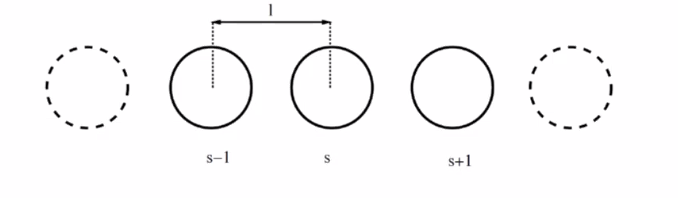
\includegraphics[scale=1]{Lecture-30/l30-img1.png}
\end{center}
\begin{s}
Since $F = kx$, if $x \mapsto \frac{x}{2}$, then $k \mapsto 2k$ in order to give the same force between the particles as the original configuration. 
\end{s}
\begin{itemize}
    \item So another condition on our limit; we will take $k \rightarrow \infty$ and $l \rightarrow 0$ with $kl$ held constant.
\end{itemize}
The idea is we will go from the position of a single particle $u_s(t)$ and take it to the continuum limit of $u(x, t)$, now considering a field.
\begin{center}
    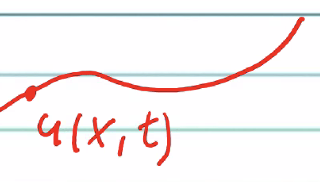
\includegraphics[scale=1]{Lecture-30/l30-img2.png}
\end{center}

\subsubsection{Deriving the Wave Equation}
Replacing the discrete positions with a continuous variable in the Newton's law equation we had in the section above, we have:
\[\dpd[2]{u(x, t)}{t} = \omega_0^2\left(u(x + l, t) + u(x - l, t) - 2u(x, t)\right)\]
But there is an issue; $\omega_0^2 = \frac{k}{m}$ diverges as $k \rightarrow \infty$ and $m \rightarrow 0$! How do we rescue this? We multiply the above equation by $1$ in a clever way, multiplying and dividing by $l^2$:
\[\dpd[2]{u(x, t)}{t} = \omega_0^2l^2\left(\frac{u(x + l, t) + u(x - l, t) - 2u(x, t)}{l}\right)\]
But this is quite convenient, as $\omega_0^2l^2 = kl\frac{l}{m} = \frac{kl}{\lambda}$ which is constant! Let us therefore denote $\omega_0^2l^2 = c^2$ where $c$ si the speed of sound. We can therefore write the above equation in the following way:
\[\dpd[2]{u(x, t)}{t} = \frac{c^2}{l}\left[\frac{u(x +l) - u(x, t)}{l} - \frac{u(x, t) - u(x - l, t)}{l}\right]\]
We recognize that the two terms in the bracket are two first order spatial derivatives. Further taking another derivative by considering the difference of the two first order derivatives by taking $l \rightarrow 0$, the RHS becomes a single second order spatial derivative:
\[\boxed{\dpd[2]{u(x, t)}{t} = c^2\dpd[2]{u(x, t)}{x}}\]
Which we recognize is a wave equation!

\subsubsection{Wave equation Solutions and Dispersion Relation}
One prime example of a solution to the wave equation is:
\[u(x, t) = A\sin(kx - \omega t)\]
Where $k$ is the wavevector and $\omega$ the frequency. Plugging this into the wave equation, we immediately obtain the (familiar) dispersion relation:
\[\omega = ck\]
Recall that in HW5 we found a relation that was slightly more complicated, and was given as:
\[\omega = 2\omega_0\abs{\sin(\frac{kl}{2})}\]
Which graphically looks like:
\begin{center}
    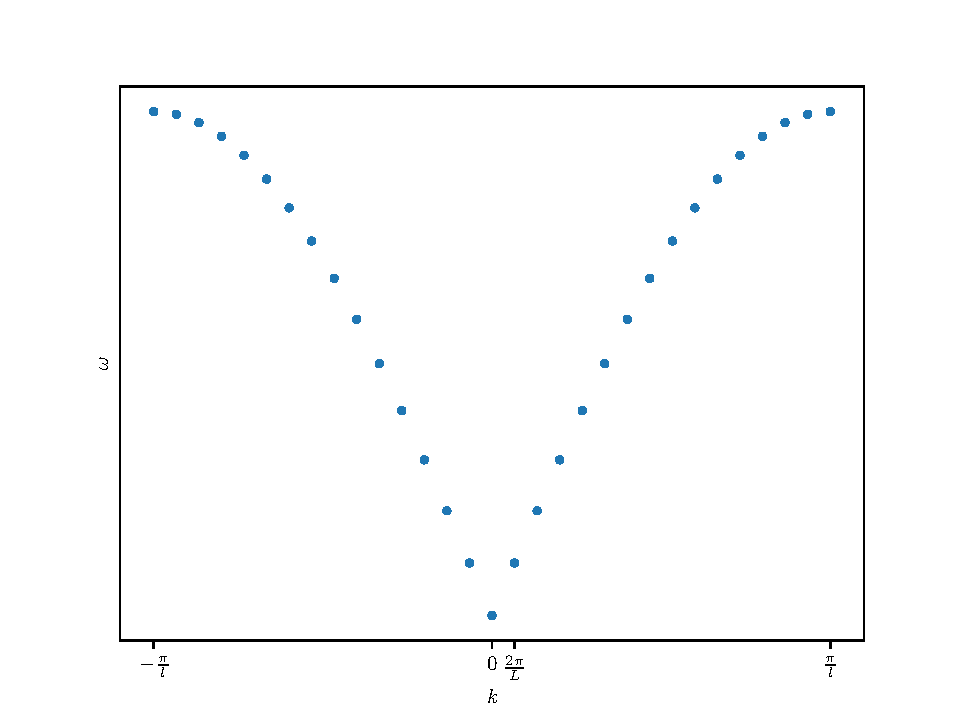
\includegraphics[scale=0.8]{Lecture-30/l30-img3.pdf}
\end{center}
So if we consider the limit of this dispersion for $kl \ll 1$, we can Taylor expand the sine and get:
\[\omega = 2\omega_0 \frac{kl}{2} = \omega_0 kl = ck\]
So we therefore have that the slope of the above graph for small $k$ is equal to $c$. We then see that we can recover the linear dispersion relationship that we obtained in the continuum limit!

\subsubsection{Generalization to 3D}
Suppose we work in three dimensions, and instead have $P = p(x, y, z)$ (pressure, or some other variable). We then have that:
\[\dpd[2]{p}{t} = c^2\left(\dpd[2]{p}{x} + \dpd[2]{p}{y} + \dpd[2]{p}{z}\right) = c^2\nabla^2 p\]
Where $\nabla^2$ is the laplacian.

\subsubsection{Volume and Surface Forces}
Since we now work with materials with a finite extension, we have more types of forces to consider. We first have \textbf{volume forces}, which are proportional to $dV$. Typical examples are gravity and electrostatic forces:
\[\v{F}_g = \rho_0 \v{g}dV\]
\[\v{F}_e = \rho_e \v{E}dV\]
$\rho_0, \rho_e$ represent mass and charge densities repectively. These are in a sense "boring" and just come from external fields.
\begin{center}
    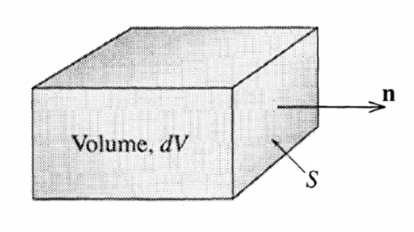
\includegraphics[scale=0.9]{Lecture-30/l30-img4.png}
\end{center}
Slightly more interesting are surface forces, which are proportional to dA. We then have Pressure, Tension, and Shear forces, as pictured below. Already things become more complicated as they depend not just on the magnitude of the force as well as the orientation of the body. 
\begin{center}
    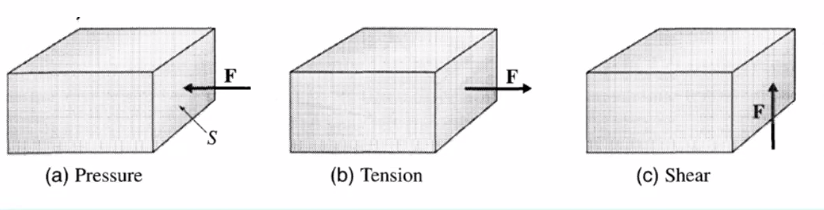
\includegraphics[scale=0.9]{Lecture-30/l30-img5.png}
\end{center}
We could of course build up to something like torsion from combinations of the above "elementary" surface forces.
\newline A question might be is where does this resistance to these surface forces come from? The answer is the intermolecular forces between the atoms in the material. 

\subsubsection{Stress \& Strain - Basic Definitions}
\begin{itemize}
    \item Stress = Force / Area = Pressure (Fluid)
    \item Stress = Tension / Area (Wire)
    \item Stress = Shear Force / Area (Shear)
    \item Strain = dV/V (Fluid)
    \item Strain = dl/l (Wire)
    \item Strain = dy/dx (Shear)
\end{itemize}
One can think of the stress as a pressure, and the Strain as a "fractional deformation"/relative change.

\subsubsection{Hooke's Law for Solids (Linear Elasticity)}
For small deformations, materials will also follow Hooke's law. We start with the wire case. If we change the wire by length $dl$, we have that the force $dF$ is given by:
\[dF = k\cdot dl\]
However, it is more useful to divide both sides by the area $A$ and add a factor of $l$ on the RHS, which gives:
\[\frac{dF}{A} = \frac{kl}{A}\frac{dl}{l}\]
Therein, the term on the LHS is the tensile stress, the rightmost term is the tensile strain (could be compressive if $dl < 0$, but let us assume for now that $dl > 0$) and define:
\[\frac{lk}{A} = Y\]
Which is Young's modulus, which is a characteristic of the material/material property. 
\newline Next, we look at a change of pressure in a fluid. We then have:
\[dp = -B\frac{dV}{V}\]
Where if we pull/expand a fluid, the pressure decreases. The $B$ is known as the bulk modulus, which tells us the response to a volumetric change (the proportionality constant to the strain). Note that in general liquids are non-compressible and hence $B$ for something like water is extremely high (but not infinite!)
\newline Finally, considering a shear, we have
\[\frac{F}{A} = G\frac{dy}{dx}\]
Where $G$ is the shear modulus. As a visual, consider shearing a material by displacing it. The amount by which we shear is $dy$. The amount of tilt is the shear strain, and the coefficient of the force that fights back is the shear modulus.
\begin{center}
    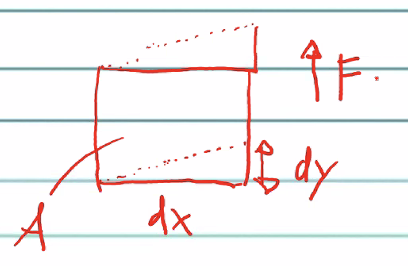
\includegraphics[]{Lecture-30/l30-img6.png}
\end{center}

\subsubsection{The Stress Tensor}
When we think of solids, we worry about two things; we both worry about the force (which has three components) as well as the orientation of the surface in which we apply the force, as the material acts differently depending along which surface we apply the force. The stress is specified by the direction of action and the orientation of the surface. This yields $3 \cdot 3 = 9$ possible components, yielding the stress tensor!
\begin{center}
    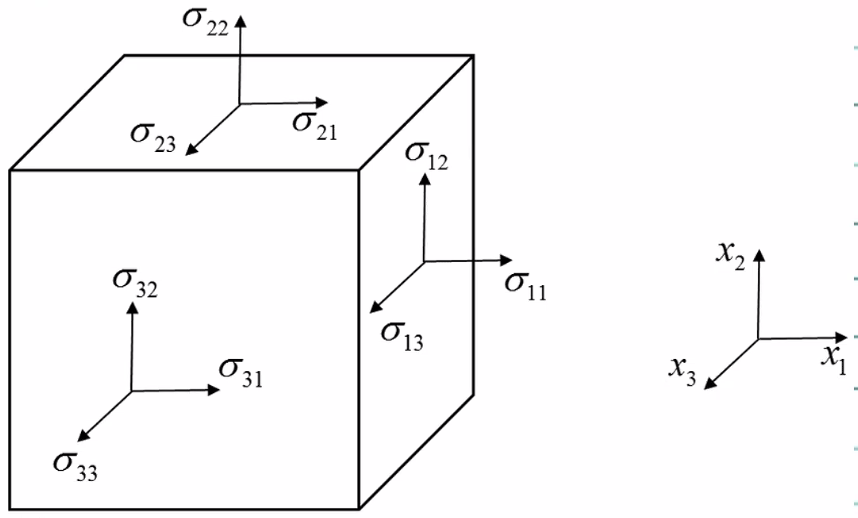
\includegraphics[scale=0.5]{Lecture-30/l30-img7.png}
\end{center}
Question: A fluid is an isotropic molecule that cannot sustain any shearing forces in equilibrium. What must be true for the stress tensor of the fluid?
\begin{s}
    The tensor must be digonal (no shear forces) with one unique component (isotropic). The idea is if we push, we feel the same pressure on all sides. There is only one scalar value which quantifies the response. For the fluid, the stress tensor will have a simple form:
    \[\sigma = \m{-P & 0 & 0 \\ 0 & -P & 0 \\ 0 & 0 & -P}, \quad  \sigma_{ij} = -P\delta_{ij}\]
    Note that this is not true of all liquids, e.g. with viscous liquids like honey we can expect shear forces when we stir.
\end{s}
Next day we will look at the counterpart of the stress tensor, the strain tensor, and hopefully get to equations of motion that describe the motion of objects with finite extension. 